\documentclass{article}
\usepackage[utf8]{inputenc}
\usepackage[left=1.0cm,right=1.0cm, top=1.5cm, bottom=1.5cm]{geometry}
\usepackage{graphicx}
\usepackage{graphics}
\usepackage{caption}
\usepackage{float}
\usepackage{amsmath}
\usepackage{amssymb}
\usepackage{amsthm}
\usepackage{listings}
\usepackage{mathtools}
\usepackage{hyperref}

% Align all equations left:
\documentclass[fleqn]{article} 

% Plot functions
\usepackage{tikz}
\usepackage{pgfplots}
\usetikzlibrary{datavisualization}
\usetikzlibrary{arrows}
\tikzstyle{int}=[draw, fill=blue!20, minimum size=2em]
\tikzstyle{init} = [pin edge={to-,thin,black}]

% Sets and quantifiers
\newcommand{\R}{\mathbb{R}\;}
\newcommand{\Q}{\mathbb{Q}\;}
\newcommand{\N}{\mathbb{N}\;}
\newcommand{\nin}{n \in \mathbb{N}}
\newcommand{\fa}{\;\forall\;}
\newcommand{\ex}{\;\exists\;}
\newcommand{\nex}{\;\nexists\;}

% Sequences
\newcommand{\seq}[1]{\{#1\}}
\newcommand{\seqx}{\seq{x_n}}
\newcommand{\seqy}{\seq{y_n}}
\newcommand{\seqs}{\seq{s_n}}

% Subsequences
\newcommand{\seqxni}{\seq{x_{n_i}}}
\newcommand{\seqyni}{\seq{y_{n_i}}}
\newcommand{\xni}{x_{n_i}}
\newcommand{\yni}{y_{n_i}}
\newcommand{\xnij}{x_{n_{i_j}}}
\newcommand{\ynij}{y_{n_{i_j}}}
\newcommand{\seqxnij}{\seq{x_{n_{i_j}}}}
\newcommand{\seqynij}{\seq{y_{n_{i_j}}}}

% Such that
\newcommand{\st}{\;\text{such that}\;}

% Vectors
\newcommand{\xhat}{\hat{\mathbf{x}}}
\newcommand{\yhat}{\hat{\mathbf{y}}}
\newcommand{\zhat}{\hat{\mathbf{z}}}
\newcommand{\nhat}{\hat{\mathbf{n}}}
\newcommand{\shat}{\hat{\mathbf{s}}}
\newcommand{\rhat}{\hat{\mathbf{r}}}
\newcommand{\vhat}{\hat{\mathbf{v}}}
\newcommand{\hatvector}[1]{\hat{\mathbf{1}}}
\newcommand{\mb}[1]{\mathbf{#1}}

% Derivatives
\newcommand{\der}[2]{\frac{d #1}{d #2}}
\newcommand{\dder}[2]{\frac{d^2 #1}{d #2^2}}
\newcommand{\derop}[1]{\frac{d}{d #1}}
\newcommand{\dderop}[1]{\frac{d^2}{d #1^2}}

% Partial Derivatives
\newcommand{\pd}[2]{\frac{\partial #1}{\partial #2}}
\newcommand{\pdd}[2]{\frac{\partial^2 #1}{\partial #2^2}}
\newcommand{\pdop}[1]{\frac{\partial}{\partial #1}}
\newcommand{\pddop}[1]{\frac{\partial^2}{\partial #1^2}}
\newcommand{\pddmixed}[3]{\frac{\partial^2 #1}{\partial #2\partial #3}}
\newcommand{\pddmixedop}[2]{\frac{\partial^2}{\partial #1\partial #2}}

% For convolution symbol
\usepackage{amssymb}

% Fourier Transform pairs
\newcommand{\ftpair}{\xleftrightarrow{\mathcal{F}}}

% ith
\newcommand{\ith}{\text{i}^{\text{th}}}

% lim, limsup, liminf
\newcommand{\limn}{\text{lim}_{n \rightarrow \infty}}
\newcommand{\limi}{\text{lim}_{i \rightarrow \infty}}
\newcommand{\limj}{\text{lim}_{j \rightarrow \infty}}
\newcommand{\limsupn}{\limsup_{n \rightarrow \infty}}
\newcommand{\liminfn}{\liminf_{n \rightarrow \infty}}

% Parallel symbols
\newcommand{\parallelsum}{\mathbin{\!/\mkern-5mu/\!}}




% Custom for absolute value
\delimitershortfall-1sp
\newcommand\abs[1]{\left|#1\right|}

% Reference and hyperlink
\newcommand{\source}[1]{\href{#1}{(\textbf{Source})}}

% Use for define equals
\newcommand{\delteq}{\overset{\Delta}{=}}

% For nicer fonts
\usepackage{eucal}

% For Dreamer Paper
\newcommand{\stau}{s_{\tau}}
\newcommand{\expect}[1]{\mathbb{E}_{#1}}
\newcommand{\indep}{\perp \!\!\! \perp}


\title{6.801/6.866: Machine Vision, Lecture 16}
\author{Professor Berthold Horn, Ryan Sander, Tadayuki Yoshitake \\
        MIT Department of Electrical Engineering and Computer Science \\ 
        Fall 2020}
\date{}

\begin{document}

\maketitle
These lecture summaries are designed to be a review of the lecture.  Though I do my best to include all main topics from the lecture, the lectures will have more elaborated explanations than these notes.  Therefore, if you're looking for the most rigorous review and treatment of these topics, we encourage you to rewatch the lecture videos.  With that said, we hope these summaries are beneficial for your learning.  If you have any feedback for these lecture summaries, please submit it \textbf{\href{https://forms.gle/itCUtP4AubAbtwQT9}{here}}.
\section{Lecture 16: Fast Convolution, Low Pass Filter Approximations, Integral Images, (US 6,457,032)}
\subsection{Sampling and Aliasing}
Sampling is a ubiquitous operation for machine vision and general signal processing.  Recall that PatMax, for instance, uses sampling in its methodology.  PatMax also performs an interesting operation: low-pass filtering before sampling.  Why is this performed?  To answer this question, let us revisit the \textbf{Nyquist Sampling Theorem}.
\subsubsection{Nyquist Sampling Theorem}
Before we dive into the mathematics behind this theorem, let us first build some intuition surrounding this theory.
\begin{itemize}
    \item If we can sample a signal at a high enough frequency, we can recover the signal exactly through reconstruction.
    \item How is this reconstruction performed?  We will convolve samples from the signal with sinc functions, and then superimpose these convolved results with one another.
    \item It is hard to sample from a signal with infinite support.
    \item What frequency do we need for this?  Intuitively, to pick out how fast the signal needs to be moving, we certainly need to sample as quickly as the signal's fastest-varying component itself.  But do we need to sample even faster?  It turns out the answer is yes.  As we will see below:
    \begin{align*}
        f_{\text{max}} < \frac{f_{\text{sample}}}{2} \implies f_{\text{sample}} > 2f_{\text{max}} &&
    \end{align*}
    I.e. we will need to sample at more than twice the frequency of the highest-varying component of the signal.
\end{itemize}
Let us look at this graphically.  What happens if we sample at the frequency of the signal?
\begin{center}
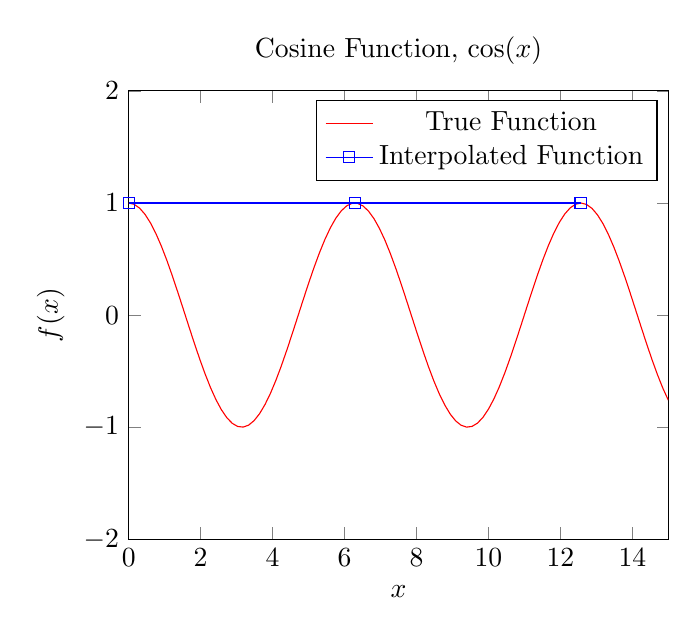
\begin{tikzpicture}
\begin{axis}[
title={Cosine Function, $\cos(x)$},
    xlabel={$x$},
    ylabel={$f(x)$},
    xmin=0, xmax=15, 
    ymin=-2, ymax=2]
\addplot[color=red, domain=0:15, samples=100]{cos(180*x/pi)};
\addlegendentry{True Function}
\addplot[
    color=blue,
    mark=square,
    ]
    coordinates {
    (0,1) (6.28, 1) (12.56, 1)
    };
\addlegendentry{Interpolated Function}
\end{axis}
\end{tikzpicture}
\captionof{figure}{Sampling only once per period provides us with a constant interpolated function, from which we cannot recover the original.  Therefore, we must sample at a higher frequency.}
\end{center}
Note that this holds at points not on the peaks as well:
\begin{center}
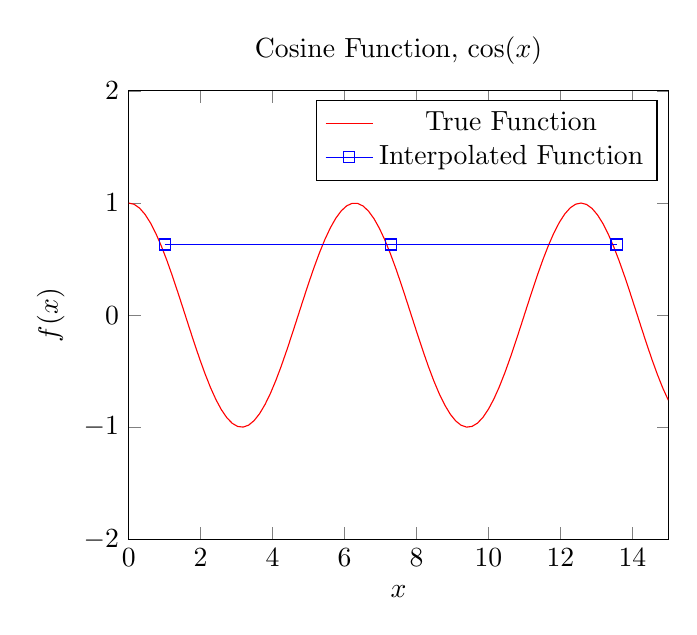
\begin{tikzpicture}
\begin{axis}[
title={Cosine Function, $\cos(x)$},
    xlabel={$x$},
    ylabel={$f(x)$},
    xmin=0, xmax=15, 
    ymin=-2, ymax=2]
\addplot[color=red, domain=0:15, samples=100]{cos(180*x/pi)};
\addlegendentry{True Function}
\addplot[
    color=blue,
    mark=square,
    ]
    coordinates {
    (1,0.63) (7.28, 0.63) (13.56, 0.63)
    };
\addlegendentry{Interpolated Function}
\end{axis}
\end{tikzpicture}
\captionof{figure}{Sampling only once per period provides us with a constant interpolated function, from which we cannot recover the original.  Therefore, we must sample at a higher frequency.}
\end{center}
What if we sample at twice the frequency?  I.e. peaks and troughs:
\begin{center}
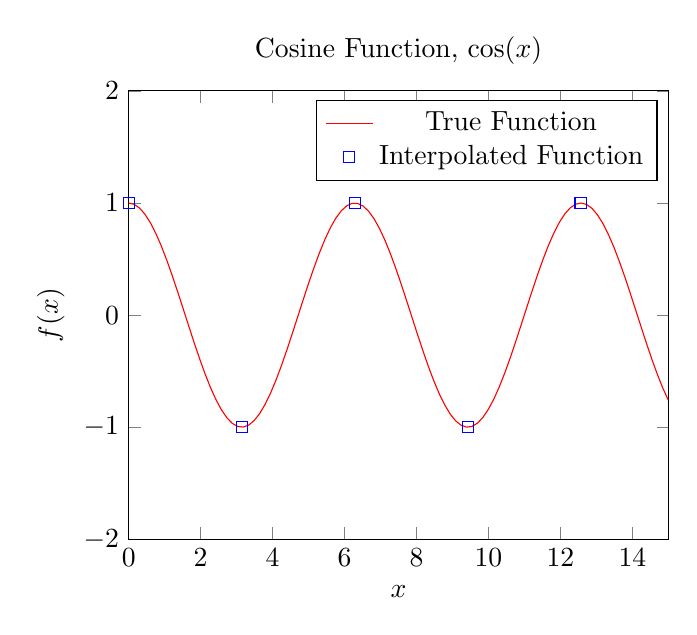
\begin{tikzpicture}
\begin{axis}[
title={Cosine Function, $\cos(x)$},
    xlabel={$x$},
    ylabel={$f(x)$},
    xmin=0, xmax=15, 
    ymin=-2, ymax=2]
\addplot[color=red, domain=0:15, samples=100]{cos(180*x/pi)};
\addlegendentry{True Function}
\addplot[
    only marks,
    color=blue,
    mark=square,
    ]
    coordinates {
    (0,1) (6.28, 1) (12.56, 1) (3.14, -1) (9.42, -1)
    };
\addlegendentry{Interpolated Function}
\end{axis}
\end{tikzpicture}
\captionof{figure}{Sampling at twice the rate as the highest-varying component almost gets us there!  This is known as the \textbf{Nyquist Rate}.  It turns out we need to sample at frequencies that are strictly greater than this frequency to guarantee no aliasing - we will see why in the example below.}
\end{center}
Is this good enough?  As it turns out, the inequality for Nyquist's Sampling Theorem is there for a reason: we need to sample at \textbf{greater than} twice the frequency of the original signal in order to uniquely recover it:
\begin{center}
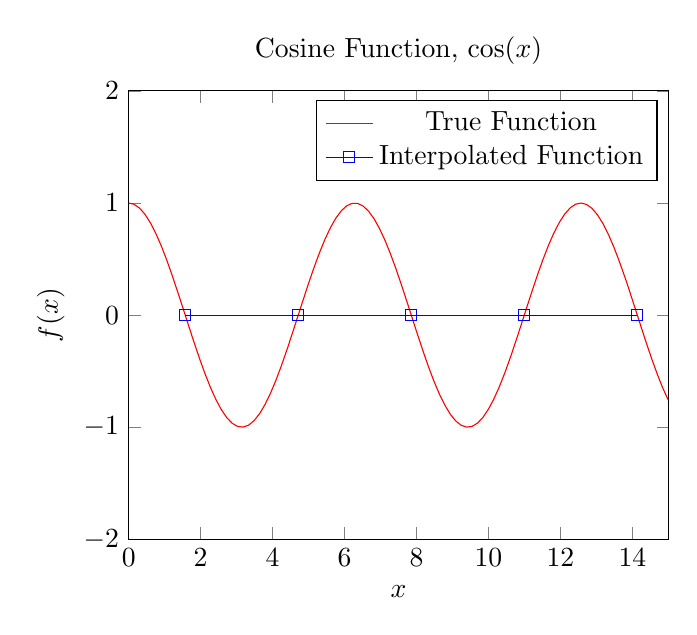
\begin{tikzpicture}
\begin{axis}[
title={Cosine Function, $\cos(x)$},
    xlabel={$x$},
    ylabel={$f(x)$},
    xmin=0, xmax=15, 
    ymin=-2, ymax=2]
\addplot[color=red, domain=0:15, samples=100]{cos(180*x/pi)};
\addlegendentry{True Function}
\addplot[
    color=blue,
    mark=square,
    ]
    coordinates {
    (1.57, 0) (4.71, 0) (7.85, 0) (10.99, 0) (14.13, 0)
    };
\addlegendentry{Interpolated Function}
\end{axis}
\end{tikzpicture}
\captionof{figure}{It turns out we need to sample at frequencies that are strictly greater than this frequency to guarantee no aliasing - we will see why in the example below.}
\end{center}
Therefore, any rate above 2 times the highest-varying frequency component of the signal will be sufficient to completely avoid aliasing.  As a review, let us next discuss aliasing.
\subsubsection{Aliasing}
Aliasing occurs when higher frequencies become indistinguishable from lower frequencies, and as a result they add interference and artifacts to the signal that are caused by sampling at too low of a frequency. \\ \\
Suppose we have a signal given by:
\begin{align*}
    f(x) = \cos(2\pi f_0x) &&
\end{align*}
And suppose we sample this signal with frequency given by $f_s = \frac{1}{\delta}$.  Then our sampled signal is given by:
\begin{align*}
    s_k = \cos(2\pi f_0 k \frac{1}{\delta}) = \cos(2\pi \frac{f_0}{f_s}k) \fa k \in \{1, 2, ...\} &&
\end{align*}
Now let us consider what happens when we add multiples of $2\pi$ to this:
\begin{align*}
    s_{k - 2\pi} & = \cos\Big(2\pi\frac{f_0}{f_s}k - 2\pi k\Big) \\
                 & = \cos\Big(2\pi\Big(\frac{f_0}{f_s} - 1\Big)k\Big) \\
                 & = \cos\Big(2\pi\Big(\frac{f_0-f_s}{f_s}\Big)k\Big) \\
                 & = \cos\Big(2\pi\Big(\frac{f_s-f_0}{f_s}\Big)k\Big), \;\; \text{since} \; \cos(x) = \cos(-x) \fa x \in \R&&
\end{align*}
Another way to put this - you cannot distinguish multiples of base frequencies with the base frequencies themselves if you sample at too low a frequency, i.e. below the \textbf{Nyquist Rate}.
\subsubsection{How Can We Mitigate Aliasing?}
There are several strategies to mitigate aliasing effects:
\begin{itemize}
    \item (Note) Anti-aliasing measures must be taken before sampling.  After sampling occurs, information is ``lost", so to speak, and the original signal cannot be recovered.
    \item High frequency noise suppression with (approximate) low-pass filtering.  As it turns out, exact lowpass filtering is impossible due to convergence properties of Fourier Series at cutoff frequencies (a phenomenon known as the \textbf{Gibbs Phenomenon} [1].
\end{itemize}
We will touch more on these anti-aliasing techniques and strategies throughout this lecture.
\subsection{Integral Image}
Next, we will shift gears somewhat to discuss the notion of an \textbf{integral image}, and the critical role this technique plays in improving computational efficiency in image processing and machine vision. We will disucss this concept in both 1D and 2D.
\subsubsection{Integral Images in 1D}
\textbf{Block averaging} is a common operation in computer vision in which we take the average over a set of values across an entire vector (1D) or matrix (2D), such as an image.  This involves summing and then dividing by the total number of elements, which can become prohibitively computationally-expensive, particularly if this operation is being called many times and the averages that we need to compute are very large.  Is there a more computationally-efficient way to do this?  \\ \\
It turns out this computationally-simpler solution is through integral images.  An integral image is essentially the sum of values from the first value to the $\ith$ value, i.e if $g_i$ defines the $\ith$ value in 1D, then:
\begin{align*}
    G_i \delteq \sum_{k=1}^{i}g_k \fa i \in \{1, \cdots, K\} &&
\end{align*}
Why is this useful?  Well, rather than compute averages (normalized sums) by adding up all the pixels and then dividing, we simply need to perform a single subtraction between the integral image values (followed by a division by the number of elements we are averaging).  For instance, if we wanted to calculate the average of values between $i$ and $j$, then:
\begin{align*}
    \bar{g}_{[i,j]} = \frac{1}{j-i}\sum_{k=i}^{j}g_k = \frac{1}{j-i}(G_j - G_i) &&
\end{align*}
This greatly reduces the amortized amount of computation, because these sums only need to be computed once, when we calculate the initial values for the integral image.
\subsubsection{Integral Images in 2D}
Now, we can extend the notion of an integral image to 2D!  Note further that integral ``images" can extend beyond images!  E.g. these can be done with gradients, Jacobians, Hessians, etc. One example in particular is calculating a Histogram of Gradients (HoG), which is quite useful for feature matching algorithms such as Scale-Invariant Feature Transform (SIFT).   These approaches also map nicely onto GPUs, enabling for even faster computation times.  \\ \\
Let us now see how block averaging looks in 2D - in the diagram below, we can obtain a block average for a group of pixels in the 2D range $(i,j)$ in $x$ and $(k,l)$ in $y$ using the following formula:
\begin{align*}
    \bar{g}_{([i,j], [k,l])} = \frac{1}{(j-i)(l-k)}\sum_{x=i}^{j}\sum_{y=k}^{l}g_{x,y} &&
\end{align*}
But can we implement this more efficiently?  We can use integral images again:
\begin{align*}
    G_{i,j} = \sum_{k=1}^{i}\sum_{l=1}^{j}g_{k,l} &&
\end{align*}
Referencing the figure below, this becomes:
\begin{figure}[ht]
    \centering
    \includegraphics[width=2\textwidth/3]{figures/2d_block_averaging.png}
    \caption{Block averaging using integral images in 2D.  As pointed out above, block averaging also extends beyond pixels!  This can be computed for other measures such as gradients (e.g. Histogram of Gradients).}
    \label{fig:my_label}
\end{figure}

Using the integral image values, the block average in the 2D range $(i,j)$ in $x$ and $(k,l)$ in $y$ becomes:
\begin{align*}
    \bar{g}_{([i,j], [k,l])} = \frac{1}{(j-i)(l-k)}\Big((G_{j,l} + G_{i,k}) - (G_{i,l} + G_{j,k})\Big) && 
\end{align*}
Some comments about this:
\begin{itemize}
    \item This analysis can be extended to higher dimensions as well!  Though the integral image will take longer to compute, and the equations for computing these block averages become less intuitive, this approach generalizes to arbitrary dimensions.
    \item As we saw in the one-dimensional case, here we can also observe that after computing the integral image (a one-time operation that can be amortized), the computational cost for averaging each of these 2D blocks becomes \textbf{independent of the size of the block being averaged}.  This stands in stark contrast to the naive implementation - here, the computational cost scales quadratically with the size of the block being averaged (or linearly in each dimension, if we take rectangular block averages).
    \item Why is this relevant?  Recall that block averaging implements approximate lowpass filtering, which can be used as a frequency suppression mechanism to avoid aliasing when filtering.
    \item In other domains outside of image processing, the integral image is known as the ``Summed-area Table" [2].
\end{itemize}
Since we intend to use this for approximate lowpass filtering, let us now change topics toward fourier analysis of this averaging mechanism to see how efficacious it is.
\subsection{Fourier Analysis of Block Averaging}
Let us consider a one-dimensional ``filter" that implements an approximate lowpass filtering for  mechanism through block averaging.  Let us consider a function such that it takes 0 value outside of the range $(-\frac{-\delta}{2}, \frac{\delta}{2})$, and value $\frac{1}{\delta}$ inside this range:
\begin{align*}
    h(x) = \begin{cases}
            \frac{1}{\delta} & x \in (-\frac{-\delta}{2}, \frac{\delta}{2}) \\
            0 & \text{o.w.}
           \end{cases}
\end{align*}
Visually:
\begin{center}
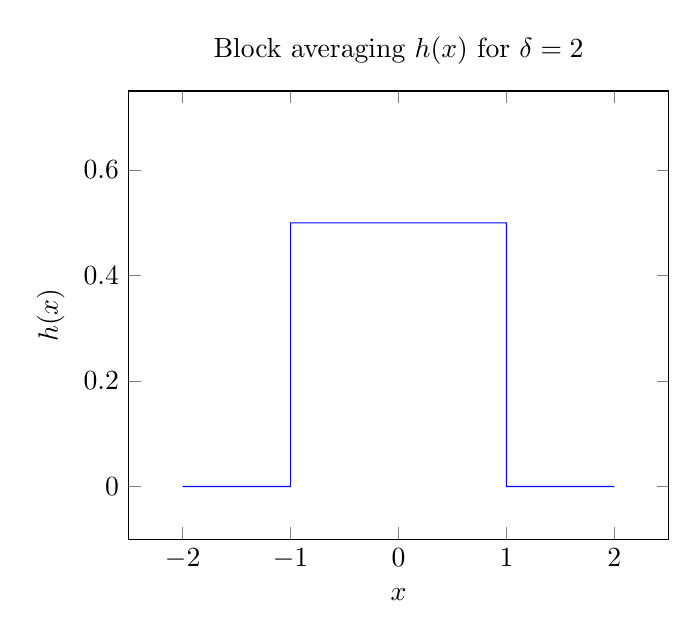
\begin{tikzpicture}
\begin{axis}[
title={Block averaging $h(x)$ for $\delta = 2$},
    xlabel={$x$},
    ylabel={$h(x)$},
    xmin=-2.5, xmax=2.5, 
    ymin=-0.1, ymax=0.75]
\addplot[
    color=blue,
    mark=none,
    ]
    coordinates {
    (-2, 0) (-1.000001, 0) (-1, 1/2) (0, 1/2) (1, 1/2) (1.0000001, 0) (2, 0)
    };
\end{axis}
\end{tikzpicture}
\captionof{figure}{Example $h(x)$ for $\delta = 2$.}
\end{center}
Let's see what this Fourier Transform looks like.  Recall that the Fourier Transform (up to a constant scale factor, which varies by domain) is given by:
\begin{align*}
    F(j\omega) = \int_{-\infty}^{\infty}f(x)e^{-j\omega x}dx &&
\end{align*}
Where $j\omega$ corresponds to complex frequency.  Substituting our expression into this transform:
\begin{align*}
    H(j\omega) & = \int_{-\infty}^{\infty}h(x)e^{-j\omega x}dx \\ \\
               & = \int_{-\frac{\delta}{2}}^{\frac{\delta}{2}}\frac{1}{\delta}e^{-j\omega x}dx \\ \\
               & = \frac{1}{\delta}\frac{1}{j\omega}[e^{-j\omega x}]_{x=-\frac{\delta}{2}}^{x=\frac{\delta}{2}} \\ \\
               & = \frac{e^{-\frac{j\omega\delta}{2}} - e^{\frac{j\omega\delta}{2}}}{-j\omega\delta} \\ \\
               & = \frac{\sin\Big(\frac{\delta\omega}{2}\Big)}{\frac{\delta\omega}{2}} \;\;\textbf{(Sinc function)}
\end{align*}
Where in the last equality statement we use the identity given by:
\begin{align*}
    \sin(x) = \frac{e^{jx}-e^{-jx}}{-2j}
\end{align*}
Graphically, this sinc function appears (for $\delta=2$):
\begin{center}
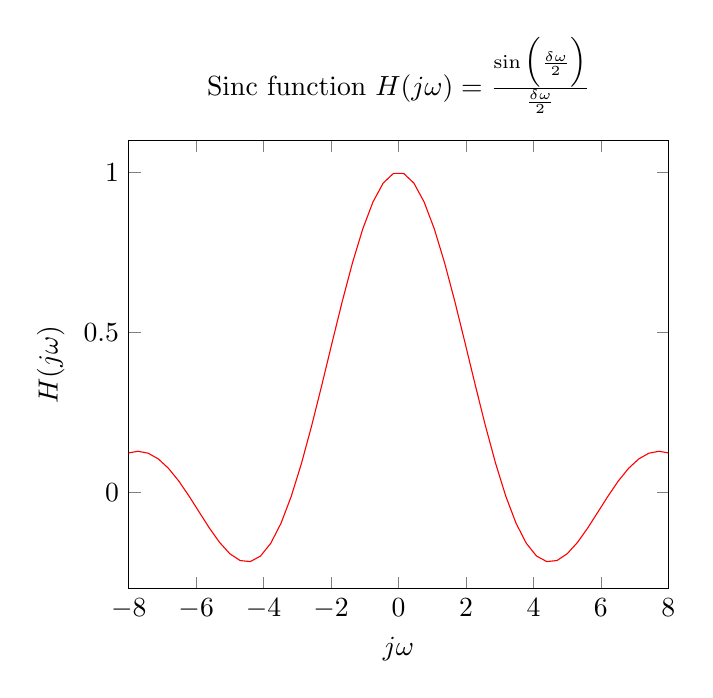
\begin{tikzpicture}
\begin{axis}[
title={Sinc function $H(j\omega) = \frac{\sin\Big(\frac{\delta\omega}{2}\Big)}{\frac{\delta\omega}{2}}$},
    xlabel={$j\omega$},
    ylabel={$H(j\omega)$},
    xmin=-8, xmax=8, 
    ymin=-0.3, ymax=1.1]
\addplot[color=red, domain=-15:15, samples=100]{sin(180*x/pi)/x};
\end{axis}
\end{tikzpicture}
\captionof{figure}{Example $H(j\omega)$ for $\delta = 2$.  This is the Fourier Transform of our block averaging ``filter".}
\end{center}
Although sinc functions in the frequency domain help to attenuate higher frequencies, they do not make the best lowpass filters.  This is the case because:
\begin{itemize}
    \item Higher frequencies are not completely attenuated.
    \item The first zero is not reached quickly enough.  The first zero is given by:
    \begin{align*}
        \frac{\omega_0\delta}{2} = \frac{\pi}{2} \implies \omega_0 = \frac{\pi}{\delta}
    \end{align*}
\end{itemize}
Intuitively, the best lowpass filters perfectly preserve all frequencies up to the cutoff frequencies, and perfectly attenuate everything outside of the passband.  Visually:
\begin{center}
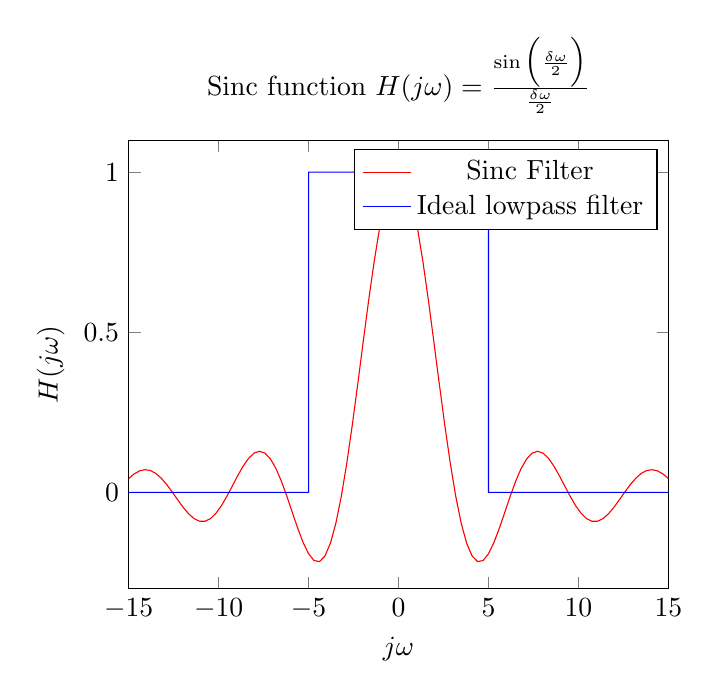
\begin{tikzpicture}
\begin{axis}[
title={Sinc function $H(j\omega) = \frac{\sin\Big(\frac{\delta\omega}{2}\Big)}{\frac{\delta\omega}{2}}$},
    xlabel={$j\omega$},
    ylabel={$H(j\omega)$},
    xmin=-15, xmax=15, 
    ymin=-0.3, ymax=1.1]
\addplot[color=red, domain=-15:15, samples=100]{sin(180*x/pi)/x};
\addlegendentry{Sinc Filter}
\addplot[
    color=blue,
    mark=none,
    ]
    coordinates {
    (-15, 0) (-5.000001, 0) (-5, 1) (0, 1) (5, 1) (5.0000001, 0) (15, 0)
    };
\addlegendentry{Ideal lowpass filter}
\end{axis}
\end{tikzpicture}
\captionof{figure}{Frequency response comparison between our block averaging filter and an ideal lowpass filter.  We also note that the ``boxcar" function and the sinc function are Fourier Transform pairs!}
\end{center}
Although sinc functions in the frequency domain help to attenuate higher frequencies, they do not make the best lowpass filters.  This is the case because:
\begin{itemize}
    \item Higher frequencies are not completely attenuated.
    \item The first zero is not reached quickly enough.  The first zero is given by:
    \begin{align*}
        \frac{\omega_0\delta}{2} = \frac{\pi}{2} \implies \omega_0 = \frac{\pi}{\delta}
    \end{align*}
\end{itemize}
Where else might we see this?  It turns out cameras perform block average filtering because pixels have finite width over which to detect incident photons.  But is this a sufficient approximate lowpass filtering technique?  Unfortunately, oftentimes it is not.  We will see below that we can improve with \textbf{repeated block averaging}.
\subsection{Repeated Block Averaging}
One way we can improve our ability to attenuate higher frequencies - repeated block averaging!  If our ``boxcar" filter given above is given by $b(x)$ (note that this was $h(x)$ above), then our previous result $y(x)$ can be written as:
\begin{align*}
    y_1(x) = f(x) \otimes b(x)
\end{align*}
\begin{center}
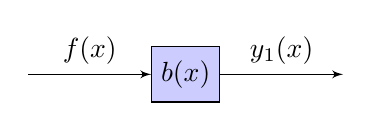
\begin{tikzpicture}[node distance=2.5cm,auto,>=latex']
    \node [int] (a) {$b(x)$};
    \node (b) [left of=a,node distance=2cm, coordinate] {a};
    \node [coordinate] (end) [right of=a, node distance=2cm]{};
    \path[->] (b) edge node {$f(x)$} (a);
    \draw[->] (a) edge node {$y_1(x)$} (end) ;
\end{tikzpicture}
\end{center}
What happens if we add another filter?  Then, we simply add another element to our convolution:
\begin{align*}
    y_2(x) = (f(x) \otimes b(x)) \otimes b(x) = y_1(x) \otimes b(x)
\end{align*}
\begin{center}
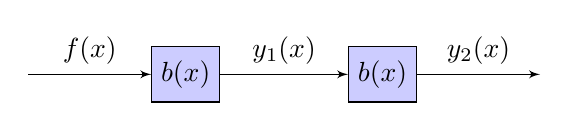
\begin{tikzpicture}[node distance=2.5cm,auto,>=latex']
    \node [int] (a) {$b(x)$};
    \node (b) [left of=a,node distance=2cm, coordinate] {a};
    \node [int] (c) [right of=a] {$b(x)$};
    \node [coordinate] (end) [right of=c, node distance=2cm]{};
    \path[->] (b) edge node {$f(x)$} (a);
    \path[->] (a) edge node {$y_1(x)$} (c);
    \draw[->] (c) edge node {$y_2(x)$} (end) ;
\end{tikzpicture}
\end{center}
Adding this second filter is equivalent to convolving our signal with the convolution of two ``boxcar" filters, which is a triangular filter:
\begin{center}
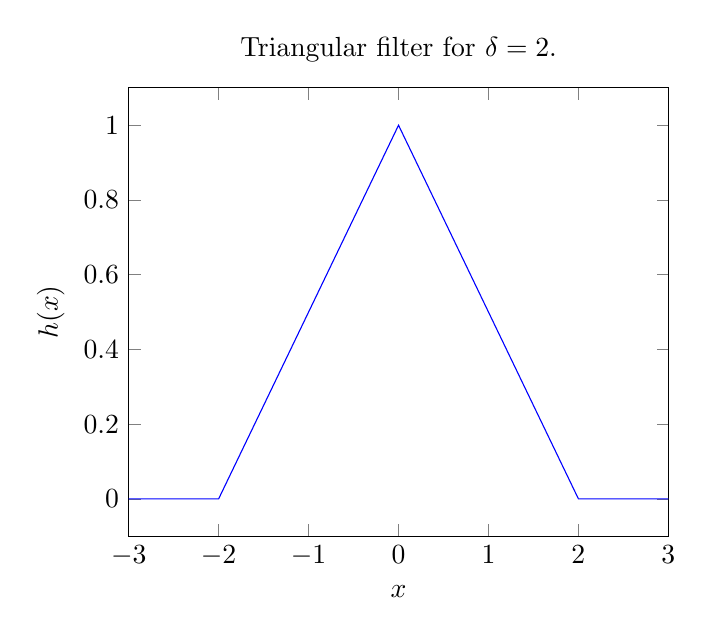
\begin{tikzpicture}
\begin{axis}[
title={Triangular filter for $\delta = 2$.},
    xlabel={$x$},
    ylabel={$h(x)$},
    xmin=-3, xmax=3, 
    ymin=-0.1, ymax=1.1]
\addplot[
    color=blue,
    mark=none,
    ]
    coordinates {
    (-3, 0) (-2, 0) (0, 1) (2, 0) (3, 0)
    };
\end{axis}
\end{tikzpicture}
\captionof{figure}{Example of a triangular filter resulting from the convolution of two ``boxcar" filters.}
\end{center}
Additionally, note that since convolution is associative, for the ``two-stage" approximate lowpass filtering approach above, we do not need to convolve our input $f(x)$ with two ``boxcar" filters - rather, we can convolve it directly with our trinagular filter $b_2(x) = b(x) \otimes b(x)$:
\begin{align*}
    y_2(x) & = (f(x) \otimes b(x)) \otimes b(x) \\
           & = f(x) \otimes (b(x) \otimes b(x)) \\
           & = f(x) \otimes b_2(x)
\end{align*}
Let us now take a brief aside to list out how discontinuities affect Fourier Transforms in the frequency domains:
\begin{itemize}
    \item \textbf{Delta Function}: $\delta(x) \ftpair 1$ \\ \\
    \textbf{Intuition}: Convolving a function with a delta function does not affect the transform, since this convolution simply produces the function.
    \item \textbf{Unit Step Function}: $u(x) \ftpair \frac{1}{j\omega}$ \\ \\
    \textbf{Intuition}: Convolving a function with a step function produces a degree of averaging, reducing the high frequency components and therefore weighting them less heavily in the transform domain.
    \item \textbf{Ramp Function}: $r(x) \ftpair -\frac{1}{\omega^2}$ \\ \\
    \textbf{Intuition}: Convolving a function with a ramp function produces a degree of averaging, reducing the high frequency components and therefore weighting them less heavily in the transform domain.
    \textbf{Derivative}: $\frac{d}{dx}f(x) \ftpair j\omega F(j\omega)$ \\ \\
    \textbf{Intuition}: Since taking derivatives will increase the sharpness of our functions, and perhaps even create discontinuities, a derivative in the spatial domain corresponds to multiplying by $j\omega$ in the frequency domain.  
\end{itemize}
As we can see from above, the more ``averaging" effects we have, the more the high-frequency components of the signal will be filtered out.  Conversely, when we take derivatives and create discontinuities in our spatial domain signal, this increases high frequency components of the signal because it introduces more variation. \\ \\
To understand how we can use repeated block averaging in the Fourier domain, please recall the following special properties of Fourier Transforms:
\begin{enumerate}
     \item \textbf{Convolution in the spatial domain corresponds to multiplication in the frequency domain}, i.e. for all $f(x), g(x), h(x)$ with corresponding Fourier Transforms $F(j\omega), G(j\omega), H(j\omega)$, we have:
    \begin{align*}
        h(x) = f(x) \otimes g(x) \ftpair H(j\omega) = F(j\omega)G(j\omega)
    \end{align*}
    \item \textbf{Multiplication in the spatial domain corresponds to convolution in the frequency domain}, i.e. for all $f(x), g(x), h(x)$ with corresponding Fourier Transforms $F(j\omega), G(j\omega), H(j\omega)$, we have:
    \begin{align*}
        h(x) = f(x)g(x) \ftpair H(j\omega) = F(j\omega) \otimes G(j\omega)
    \end{align*}
\end{enumerate}
For block averaging, we can use the first of these properties to understand what is happening in the frequency domain:
\begin{align*}
    y_2(x) = f(x) \otimes (b(x) \otimes b(x)) \ftpair Y(j\omega) = F(j\omega)(B(j\omega)^2)
\end{align*}
This operation is equivalent to a $\text{sinc}^2$ function in the spatial domain:
\begin{center}
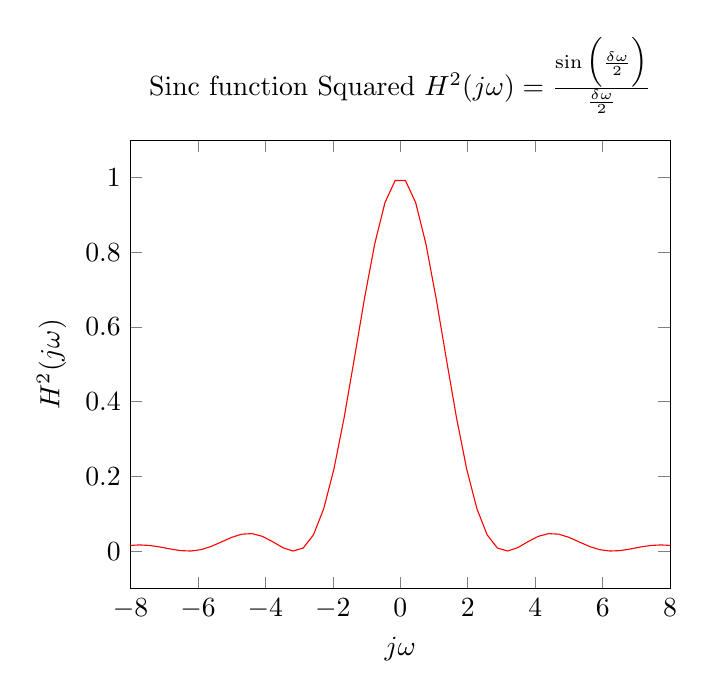
\begin{tikzpicture}
\begin{axis}[
title={Sinc function Squared $H^2(j\omega) = \frac{\sin\Big(\frac{\delta\omega}{2}\Big)}{\frac{\delta\omega}{2}}$},
    xlabel={$j\omega$},
    ylabel={$H^2(j\omega)$},
    xmin=-8, xmax=8, 
    ymin=-0.1, ymax=1.1]
\addplot[color=red, domain=-15:15, samples=100]{(sin(180*x/pi)/x)^2};
\end{axis}
\end{tikzpicture}
\captionof{figure}{Example $H^2(j\omega)$ for $\delta = 2$.  This is the Fourier Transform of our block averaging ``filter" convolved with itself in the spatial domain.}.
\end{center}
This is not perfect, but it is an improvement.  In fact, the frequencies with this filter drop off with magnitude $\Big(\frac{1}{\omega})^2$.  What happens if we continue to repeat this process with more block averaging filters?  It turns out that for $N$ ``boxcar" filters that we use, the magnitude will drop off as $\Big(\frac{1}{\omega}\Big)^N$.  Note too, that we do not want to go ``too far" in this direction, because this repeated block averaging process will also begin to attenuate frequencies in the passband of the signal.
\subsubsection{Warping Effects and Numerical Fourier Transforms: FFT and DFT}
Two main types of numerical transforms we briefly discuss are the Discrete Fourier Transform (DFT) and Fast Fourier Transform (FFT).  The FFT is an extension of the DFT that relies on using a ``divide and conquer" approach to reduce the computational runtime from $f(N) \in O(N^2)$ to $f(N) \in O(N\log N)$ [3]. \\ \\
Mathematically, the DFT is given as a transform that transforms a sequence of $N$ complex numbers $\{x_n\}_{n=1}^{N}$ into another sequence of $N$ complex numbers $\{X_k\}_{k=1}^{N}$ [4].  The transform for the $K^{\text{th}}$ value of this output sequence is given in closed-form as:
\begin{align*}
    X_k = \sum_{i=1}^{N}x_ne^{-j\frac{2\pi}{N}kn}
\end{align*}
And the inverse transform for the $n^{\text{th}}$ value of this input sequence is given as:
\begin{align*}
    x_n = \sum_{k=1}^{N}X_ke^{j\frac{2\pi}{N}kn}
\end{align*}
One aspect of these transforms to be especially mindful of is that they introduce a wrapping effect, since transform values are spread out over 2$\pi$ intervals.  This means that the waveforms produced by these transforms, in both the spatial (if we take the inverse transform) and frequency domains may be repeated - this repeating can introduce undesirable discontinuities, such as those seen in the graph below:
\begin{center}
\begin{tikzpicture}
\begin{axis}[
title={Repeated Function $x^2$},
    xlabel={$x$},
    ylabel={$f(x)$},
    xmin=0, xmax=8, 
    ymin=0, ymax=8]
\addplot[color=red, domain=0:2.5, samples=100]{x^2};
\addplot[color=red, domain=2.5:5.0, samples=100]{(x-2.5)^2};
\addplot[color=red, domain=5.0:7.5, samples=100]{(x-5.0)^2};
\end{axis}
\end{tikzpicture}
\captionof{figure}{Example of a repeated waveform that we encounter when looking at DFTs and FFTs.}
\end{center}
\textbf{Fun fact}: It used to be thought that natural images had a power spectrum (power in the frequency domain) that falls off as $\frac{1}{\omega}$.  It turns out that this was actually caused by warping effects introduced by discrete transforms. \\ \\
This begs the question - how can we mitigate these warping effects?  Some methods include:
\begin{itemize}
    \item \textbf{Apodizing}: This corresponds to multiplying your signal by a waveform, e.g. Hamming's Window, which takes the form akin to a Gaussian, or an inverted cosine.
    \item \textbf{Mirroring}: Another method to mitigate these warping effects is through waveform mirroring - this ensures continuity at points where discontinuties occurred:
    \begin{center}
    \begin{tikzpicture}
    \begin{axis}[
    title={Repeated Function $x^2$},
        xlabel={$x$},
        ylabel={$f(x)$},
        xmin=0, xmax=8, 
        ymin=0, ymax=8]
    \addplot[color=red, domain=0:2.5, samples=100]{x^2};
    \addplot[color=red, domain=2.5:5.0, samples=100]{(2.5-(x-2.5))^2};
    \addplot[color=red, domain=5.0:7.5, samples=100]{(x-5.0)^2};
    \end{axis}
    \end{tikzpicture}
    \captionof{figure}{Example of a mirrored waveform that we can use to counter and mitigate the discontinuity effects of warping from transforms such as the DFT and FFT.}
    \end{center}
    With this approach, the power spectrum of these signals falls off at $\frac{1}{\omega^2}$, rather than $\frac{1}{\omega}$.
    \item \textbf{Infinitely Wide Signal}: Finally, a less practical, but conceptual helpful method is simply to take an ``infinitely wide signal".
\end{itemize}
Let us now switch gears to talk more about the unit impulse and convolution.
\subsection{Impulses and Convolution}
In this section, we will review impulse functions, and discuss how they relate to many properties with convolution.  We will begin by reviewing delta functions and their properties.
\subsubsection{Properties of Delta Functions}
Recall that the Dirac delta function $\delta(x)$, or impulse function, is defined according to the two properties:
\begin{enumerate}
    \item \textbf{Unit Area}: $\int_{-\infty}^{\infty}\delta(x)dx = 1$
    \item \textbf{Sifting Property}: $f(x_0) = \int_{-\infty}^{\infty}f(x)\delta(x-x_0)dx$
\end{enumerate}
Another way to conceptualize delta functions is through \textbf{probabilistic distributions}.  We can use Gaussians (one of the only distributions to have a Fourier Transform).  Recall that the (zero-mean) Gaussian Fourier Transform pair is given by:
\begin{align*}
    \frac{1}{\sigma\sqrt{2\pi}}e^{-\frac{x}{2\sigma^2}} \ftpair e^{-\frac{\omega^2\sigma^2}{2}}
\end{align*}
An impulse can be conceptualized as the limit in which the variance of this Gaussian distribution $\sigma^2$ goes to 0, which corresponds to a Fourier Transform of 1 for all frequencies (which is the Fourier Transform of a delta function). \\ \\
Another way to consider impulses is that they are the limit of ``boxcar" functions as their width goes to zero. \\ \\
Let us next generalize from a single impulse function to combinations of these functions.
\subsubsection{Combinations of Impulses}
When are combinations of impulses helpful?  it turns out that one particular combination can be used for approximating the derivative using our prior work on finite differences:
\begin{align*}
    h(x) = \frac{1}{\epsilon}\Big(\delta(x + \frac{\epsilon}{2}) - \delta(x-\frac{\epsilon}{2})\Big) \;\; \text{for some} \; \epsilon > 0
\end{align*}
Correlating (*note that this is not convolution - if we were to use convolution, this derivative would be flipped) this combination of impulse ``filter" with an arbitrary function $f(x)$, we compute a first-order approximation of the derivative:
\begin{align*}
    f'(x) & \approx \int_{-\infty}^{\infty}f(x)h(x)dx \\
          & = \int_{-\infty}^{\infty}\Big(\frac{1}{\epsilon}\Big(\delta(x + \frac{\epsilon}{2}) - \delta(x-\frac{\epsilon}{2})\Big)\Big)dx
\end{align*}
Therefore, combinations of impulses can be used to represent the same behavior as the ``computational molecules" we identified before.  It turns out that there is a close connection between \textbf{linear, shift-invariant} operators and \textbf{derivative operators}. \\ \\
With impulses motivated, let us now formally review convolution.
\subsubsection{Convolution Review}
Recall from the example above that the convolution operation is simply the result of the correlation operation flipped.  Mathematically, the convolution of functions $f(x)$ and $h(x)$ is given by the following commutative operation:
\begin{align*}
    g(x) & = f(x) \otimes h(x) \\
         & = \int_{-\infty}^{\infty}f(\xi)h(x-\xi)d\xi \\
         & = h(x) \otimes g(x) \\
         & = \int_{-\infty}^{\infty}h(\xi)f(x-\xi)d\xi \\
\end{align*}
\subsubsection{Analog Filtering with Birefringent Lenses}
Why filter in the analog domain?  Returning to our original problem of mitigating aliasing artifacts through high-frequency suppression, unfortunately, if we wait to digitally filter out high frequencies after the image has already been taken by a camera or sensor, then we have already caused aliasing. \\ \\
One way to achieve this analog filtering is through \textbf{Birefringent Lenses}.  Here, we essentially take two ``shifted" images by convolving the image with a symmetric combination of offset delta functions, given mathematically by:
\begin{align*}
    h(x) = \frac{1}{2}\delta(x + \frac{\epsilon}{2}) + \frac{1}{2}\delta(x - \frac{\epsilon}{2}) \;\; \text{for some} \;\epsilon > 0
\end{align*}
Let us look at the Fourier Transform of this filter, noting the following Fourier Transform pair:
\begin{align*}
    \delta(x-x_0) \ftpair e^{-j\omega x_0}
\end{align*}
With this we can then express the Fourier Transform of this filter as:
\begin{align*}
    F(j\omega) & = \frac{1}{\sqrt{2\pi}}\int_{-\infty}^{\infty}h(x)e^{-j\omega x}dx \\
               & = \frac{1}{2}\Big(e^{-\frac{j\omega\epsilon}{2}} + e^{\frac{j\omega\epsilon}{2}}\Big) \\
               & = \cos\Big(\frac{\omega\epsilon}{2}\Big)
\end{align*}
With this framework, the first zero to appear here occurs at $\omega_0 = \frac{\pi}{\epsilon}$.  A few notes about these filters, and how they relate to high-frequency noise suppression.
\begin{itemize}
    \item When these birefringent lenses are cascaded with a \textbf{block averaging} filter, this results in a combined filtering scheme in which the zeros of the frequency responses of these filters cancel out most of the high-frequency noise.
    \item In the 2D case, we will have 2 birefringent filters, one for the x-direction and one for the y-direction.  Physically, these are rotated 90 degrees off from one another, just as they are for a 2D cartesian coordinate system.
    \item High-performance lowpass filtering requires a large \textbf{support} (see definition of this below if needed) - the computational costs grow linearly with the size of the support in 1D, and quadratically with the size of the support in 2D.  The support of a function is defined as the set where $f(\cdot)$ is nonzero [5]:
    \begin{align*}
        \text{supp}(f) = \{x: f(x) \neq 0, x \in \mathbb{R}\}
    \end{align*}
    \item Therefore, one way to reduce the computatonal costs of a filtering system is to reduce the size/cardinality of the support $|\text{supp}(f)|$ - in some sense to encourage sparsity.  Fortunately, this does not necessarily mean looking over a narrower range, but instead just considering less points overall.
\end{itemize}
\subsubsection{Derivatives and Integrals as Convolution Operators and FT Pairs}
As we have seen before, convolving a function with a unit step function results in integrating the given function.  Let us verify this below:
\begin{align*}
    f(x) \otimes u(x) & = \int_{-\infty}^{\infty}f(\xi)u(x-\xi)d\xi \\
                      & = \int_{-\infty}^{\infty}f(x-\xi)u(\xi)d\xi \\
                      & = \int_{0}^{\infty}f(\xi)d\xi
\end{align*}
Therefore, we can represent integral and derivative operators as Fourier Transform pairs too, denoted $\mathcal{S}$ for integration and $\mathcal{D}$ for derivative:
\begin{itemize}
    \item $\mathcal{S} \ftpair \frac{1}{j\omega}$
    \item $\mathcal{D} \ftpair j\omega$
\end{itemize}
Niote that we can verify this by showing that convolving these filter operators corresponds to multiplying these transforms in frequency space, which results in no effect when cascaded together:
\begin{align*}
    (f(x) \otimes \mathcal{D}) \otimes \mathcal{S} = f(x) \otimes (\mathcal{D} \otimes \mathcal{S}) \ftpair F(j\omega)\Big(j\omega \frac{1}{j\omega}\Big) = F(j\omega) \ftpair f(x)
\end{align*}
\begin{center}
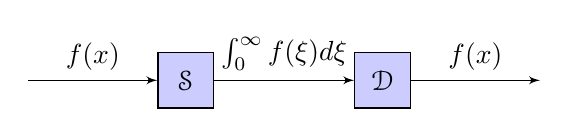
\begin{tikzpicture}[node distance=2.5cm,auto,>=latex']
    \node [int] (a) {$\mathcal{S}$};
    \node (b) [left of=a,node distance=2cm, coordinate] {a};
    \node [int] (c) [right of=a] {$\mathcal{D}$};
    \node [coordinate] (end) [right of=c, node distance=2cm]{};
    \path[->] (b) edge node {$f(x)$} (a);
    \path[->] (a) edge node {$\int_{0}^{\infty}f(\xi)d\xi$} (c);
    \draw[->] (c) edge node {$f(x)$} (end) ;
\end{tikzpicture}
\end{center}
\begin{center}
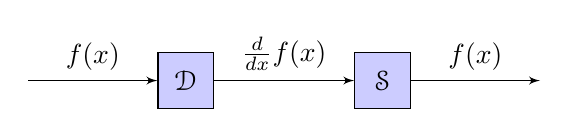
\begin{tikzpicture}[node distance=2.5cm,auto,>=latex']
\node [int] (a) {$\mathcal{D}$};
\node (b) [left of=a,node distance=2cm, coordinate] {a};
\node [int] (c) [right of=a] {$\mathcal{S}$};
\node [coordinate] (end) [right of=c, node distance=2cm]{};
\path[->] (b) edge node {$f(x)$} (a);
\path[->] (a) edge node {$\frac{d}{dx}f(x)$} (c);
\draw[->] (c) edge node {$f(x)$} (end) ;
\end{tikzpicture}
\end{center}
Can we extend this to higher-order derivatives?  It turns out we can.  One example is the convolution of two derivative operators, which becomes:
\begin{align*}
    h(x) = \delta(x+\frac{\epsilon}{2}) - 2\delta(x) + \delta(x -\frac{\epsilon}{2}) = \mathcal{D} \otimes \mathcal{D} \ftpair H(j\omega) = D(j\omega)^2 = (j\omega)^2 = -\omega^2 \;\; \text{(Recall that} \; j^2 = -1)
\end{align*}
In general, this holds.  Note that the number of integral operators $\mathcal{S}$ must be equal to the number of derivative operators $\mathcal{D}$, e.g. for $K\th$ order:
\begin{align*}
    \Big(\otimes_{i=1}^{K}\mathcal{S}\Big) \otimes \Big(\Big(\otimes_{i=1}^{K}\mathcal{D}\Big) \otimes f(x)\Big)
\end{align*}
\subsubsection{Interpolation and Convolution}
A few notes about interpolation methods:
\begin{itemize}
    \item These methods work well computationally when there is sparsity in the operators we with - for instance, cubic or linear interpolation.  Photoshop and other photo-editing software frameworks iuse this interpolation techniques.  Performance deteriorates when we switch from \textbf{cubic interpolation} to \textbf{Nearest Neighbor interpolation}.
    \item The \textbf{bicubic spline} is a popular interpolation technique.  It was invented by IBM and was used in early satellite image processing.  However, it requires many neighboring pixels, as it is composed of 7 points to interpolate over, so it is less computationally-efficient.
    \item Recall that one key element of computational efficiency we pursue is to use integral images for block averaging, which is much more efficient than computing naive sums, especially if (1) This block averaging procedure is repeated many times (the amortized cost of computing the integral image is lessened) and (2) This process is used in higher dimensions.
    \item \textbf{Linear interpolation} can be conceptualized as connecting points together using straight lines between points.  This corresponds to piecewise-linear segments, or, convolution with a triangle filter, which is simply the convolution of two ``boxcar filters":
    \begin{align*}
        f(x) = f(1)x + f(0)(1-x)
    \end{align*}
    Unfortunately, one ``not-so-great" property of convolving with triangular filters for interpolation is that the noise in the interpolated result varies depending on how far away we are from the sampled noise.
    \item \textbf{Nearest Neighbor} techniques can also be viewed through a convolutional lens - since this method produces piecewise-constant interpolation, this is equivalent to convolving our sampled points with a ``boxcar" filter!
\end{itemize}
\subsubsection{Rotationally-Symmetric Lowpass Filter in 2D}
Where $u$ and $v$ are the spatial frequencies of $x$ and $y$, i.e. the 2D Fourier Transform and Inverse Fourier Transform then take the forms of:
\begin{align*}
    & F(u,v) = \frac{1}{\sqrt{2\pi}}\int_{-\infty}^{\infty}\int_{-\infty}^{\infty}f(x,y)e^{-j(ux+vy)}dxdy \\
    & f(x,y) = \frac{1}{\sqrt{2\pi}}\int_{-\infty}^{\infty}\int_{-\infty}^{\infty}F(u,v)e^{j(ux+vy)}dudv \\
\end{align*}
The inverse transform of this can be thought of as a \textbf{sinc} function in polar coordinates:
\begin{align*}
    f(\rho, \theta) = \frac{B^2}{2\pi}\frac{J_1(\rho B)}{\rho B}
\end{align*}
A few notes about this inverse transform function:
\begin{itemize}
    \item This is the point spread function of a microscope.
    \item $J_1(\cdot)$ is a 1st-order Bessel function.
    \item This relates to our \textbf{defocusing} problem that we encountered before.
    \item In the case of defocusing, we can use the ``symmetry" property of the Fourier Transform to deduce that if we have a circular point spread function resulting from defocusing of the lens, then we will have a Bessel function in the frequency/Fourier domain.
    \item Though a pointspread function is a ``pillbox" in the ideal case, in practice this is not perfect due to artifacts such as lens aberrations.
\end{itemize}
\subsection{References}
\begin{enumerate}
    \item Gibbs Phenomenon, https://en.wikipedia.org/wiki/Gibbs\_phenomenon
    \item Summed-area Table, https://en.wikipedia.org/wiki/Summed-area\_table
    \item Fast Fourier Transform, https://en.wikipedia.org/wiki/Fast\_Fourier\_transform
    \item Discrete Fourier Transform, https://en.wikipedia.org/wiki/Discrete\_Fourier\_transform
    \item Support, https://en.wikipedia.org/wiki/Support\_(mathematics)
\end{enumerate}
\end{document}
